% com-cas
% by hk, rj, January 2012

\documentclass{llncs}

%create pdf images with epstopdf not ps2pdf

%todo:

\usepackage{epsfig}
%\usepackage{graphicx}
\usepackage{amssymb}
%\usepackage{amsmath}
%\usepackage{amsfonts}

\addtolength{\textheight}{1.5cm}

\newcommand{\code}[1]{\texttt{#1}}
\raggedbottom

\begin{document}

\title{Categories as classes with mixin composition}

\author{Heinz Kredel\inst{1} and Raphael Jolly\inst{2}} 
\institute{IT-Center, University of Mannheim, Germany,
\email{kredel@rz.uni-mannheim.de,}
\and Databeans, Paris, France,
\email{raphael.jolly@free.fr}}

\maketitle

\begin{abstract} 
  To be written
\end{abstract}

%\keywords{object oriented programming, generic type-safe library, algebraic field extensions}


\section{Introduction} %------------

To be written

\subsection{Related work} % -----------------------------------

The related work published on type systems for computer algebra or
abstract data type (ADT) approaches to computer algebra has been
summarized in \cite{JollyKredel:2010,JollyKredel:2011}.  Type-safe
design considerations in computer algebra are mostly centered around
the {\em axiom} and {\em Magma} computer algebra systems and are
described, for example in
\cite{JenksSutor:1992,Watt:2003,BosmaCannonPlayoust:1997,Stein:2005,SageWiki:2009}.
%
Further related work is mentioned in the paper as required.


\subsection{Outline} % -----------------------------------



\section{Generic, typed object oriented computer algebra software} % ----------------
\label{sec:asto}

In this section we first give an introduction into the object oriented
type systems. For more details see our earlier articles and implementations
\cite{JollyKredel:2010,Jolly:2010,Kredel:2000,Kredel:2008a,Kredel:2008}. %,Kredel:2006
Then we discuss the design and implementation of algebraic and
transcendental extension fields together with the modeling of real
algebraic and complex algebraic extension fields. The constructed
extension fields can be used in other algorithms on polynomials with
coefficients from such fields, for example in (parallel) Gr\"obner
base or greatest common divisor computations. Other algorithms like
polynomial factorization will however require an implemented case for
such fields. Due to space limitations we will not discuss performance,
but will give some hints on computing times and possible improvements.
We will also not be able to discuss mappings of elements between the
various extension rings and fields, as for example evaluation
homomorphisms between polynomial rings. Currently all such mappings
and their application have to be coded explicitly, but some automatic
mapping construction and convenient coercion would be desirable, at
least in scripting interpreters (for a special case see Subsection
? ): %\ref{sec:deptyp}).


\subsection{Ring elements and ring factories} %------------

The basic building blocks of the type system consists of the
interfaces \code{RingElem} and \code{RingFactory} and the classes
which implement them, see figure \ref{fig:bastype}. \code{RingElem}
defines the methods which we expect to be available on all ring
elements, for example \code{multiply()},
\code{isZERO()} or \code{isUnit()} with the obvious meanings. The
construction of ring elements is done by factories, modeled after the
{\em abstract factory} creational design pattern \cite{Gamma:1995}.
The factory \code{RingFactory} defines the construction methods for
elements, for example \code{get\-ONE()} to create the one element from
the ring, 
%\code{from\-Integer()} to embed the natural numbers into the ring, \code{subtract()},
%\code{random()} to create a random element 
\code{parse()} to create an element from a string representation or query methods such as
\code{is\-Asso\-ciative()}. % to query if the ring is associative. 

\begin{figure}[thb]
\centering
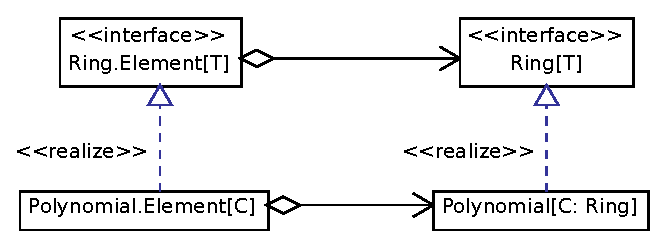
\epsfig{file=BasicTypes,clip=,width=0.7\linewidth}
%\\
\caption{Basic types}
\label{fig:bastype}
\end{figure}

The polynomial class \code{Gen\-Polynomial} with type parameter
\code{C} for the coefficient type implements the \code{Ring\-Elem}
interface and specifies that coefficients must be of type
\code{Ring\-Elem}.  In addition to the methods mandated by the
interface, the \code{Gen\-Polynomial} implements the methods like
\code{leading\-Monomial()} or \code{degree()}.  Polynomials are to be
created with a polynomial factory \code{Gen\-Polynomial\-Ring}. In
addition to the ring factory methods it defines for example methods
to create random polynomials.  The constructor for
\code{Gen\-Polynomial\-Ring} takes parameters for a factory for the
coefficients, the number of variables, the names for the variables and
a term order object \code{Term\-Order}. The relation between the
factory of the coefficients and the polynomial ring factory is modeled
after the (constructor) dependency injection pattern and implements the
inversion of control principle.

Figure \ref{fig:bastype} shows dependency arrows from the factories to
the element interfaces as factories create the respective elements.
The modeling of the constructors is not shown as it is not denotable
in Java. The constructors of ring elements implement an opposite
dependency : each constructor takes a corresponding ring
factory as parameter.  It is only indirectly enforced since the
\code{RingElem} interface specifies a method \code{factory()} to
obtain the corresponding factory.
% So methods on ring elements have access to the corresponding
% factory for construction of new elements.

The factory methods are not static (which is apparent from the
modeling as an interface) since a ring factory might depend on other
rings or specific parameters. In case of a polynomial factory it
depends on a factory for the coefficients and at least the number of
variables of the polynomial ring. By this modeling the types of
elements of algebraic structures are not simply denoted in the program
text but have to be created as programming objects (by instantiating
the respective classes). Type denotations show up explicitly in Java
program code and are mostly inferred in Scala via type resolution.

For example a polynomial $w^2 - 2 \in \mathbb{Q}[w]$ can be
constructed by first constructing an object for the ring
$\mathbb{Q}[w]$ and then reading and constructing the polynomial $w^2
- 2$ with the factory method \code{parse()}.
{\small
\begin{verbatim}
 BigRational rf = new BigRational(1); // here element = factory
 GenPolynomialRing<BigRational> pf 
  = new GenPolynomialRing<BigRational>(rf,new String[]{ "w" });
 GenPolynomial<BigRational> a = pf.parse("w^2 - 2");
\end{verbatim}
}
This example is continued in Subsection ?. %\ref{sec:anqf}.


\subsection{Algorithms and factories} %-----------------------------
\label{sec:anf}

Our implemented algorithms are in fact meta-algorithms or functors.
They do not only compute elements of algebraic structures but
simultaneously construct the required algebraic structures during
the computation.  So several implemented methods map pairs of
algebraic structures together with some elements to other algebraic
structures and elements. For example Hensel lifting is an algorithm
which maps
$$
  ((\mathbb{Z}[x],a),(\mathbb{Z}_{p}[x],(a_1,...,a_r)),(\mathbb{N},k)) 
  \mapsto 
  (\mathbb{Z}_{p^k}[x],(b_1,...,b_r)).  
$$
With the meaning
$
  (a \in \mathbb{Z}[x],(a_1,...,a_r) \in \mathbb{Z}_{p}[x]^r,k \in \mathbb{N}) 
  \mapsto 
  (b_1,...,b_r) \in \mathbb{Z}_{p^k}[x]^r.  
$
Using type annotations it would read
$$
  (a : \mathbb{Z}[x], (a_1,...,a_r): \mathbb{Z}_{p}[x]^r, k: \mathbb{N}) 
  \mapsto 
  (b_1,...,b_r) : \mathbb{Z}_{p^k}[x]^r.  
$$
It is important to understand that $\mathbb{Z}_{p^k}[x]$ is an object
constructed during the computation.  The type annotation hides this
fact.  
Note, the rings $\mathbb{Z}_{p}$ and $\mathbb{Z}_{p^k}$ are not
distinguished by a Java type. To correctly model this as distinct
types needs the concept of {\em dependent types} which is not
available in Java 6 but is available in Scala, see Subsection
?. %\ref{sec:deptyp}.


%\begin{figure}[thb]
%\centering
%\epsfig{file=AlgebraicMethods,clip=,width=0.81\linewidth}
%\\
%\caption{Methods for algebraic numbers}
%\label{fig:algmeth}
%\end{figure}


\section{Comparison with Magma and Sage} % --------------------------------
\label{sec:magma}

``Theoretical Foundations'':

{\em Universal Algebra} and order/multi sorted $\Sigma$-algebras for types,
homomorphic images of $\Sigma$-algebras, sub-$\Sigma$-algebras,
quotient $\Sigma$-algebras, direct product of $\Sigma$-algebras.

$\Sigma$-variety: $\Sigma$-algebra closed under sub-algebras,
homomorphic images, direct products (hence also closed under quotient
structures)

$\Sigma$-algebras defined by an equational theory with equations $P$ 
$\Longleftrightarrow$ variety

example the class of fields (of characteristic x) are not a variety
because they are not closed under direct products.

{\em Categories} objects (carrier sets), morphisms, and composition of morphisms.
Functors between categories, existance of free algebras (generated by a set X)
existance of generators via quotients of free algebras, 
homomorphism representation via images of generators.

{\em Magma model} {\bf magma} = $\Sigma$-algebra:
$\Sigma$-varieties (defined by equations $P$) $V = Var(\Sigma,P)$, 
categories (varieties sharing the same representation $R$) $C = Cat(V,R)$.
generic functions: $\sim$ abstract methods.
examples: groups, commutative rings, modules,

categories are concrete (no abtract parts with missing implementations) $\sim$ axiom domains.
families of categories: multivariate polynomial rings indexed by coefficient rings

compositon of categories: construction of new magmas.
category determines: representation of elements and the carrier sets, 
operations on elements and carrier sets (of a magma).

creation and deletion of magmas, elements and morphisms, mappings and coercion,
$\Sigma$-operations, representation specific operations.

constructors for magmas, elements and mappings: primitive magmas,
mappings, generators and relations (equations), S, Q, H, E, P
universal algebra constructions (ua cons).

coercions: automatic for S and Q ua cons, forced coercions $type\, !\, expression$.

{\em Magma language}



\section{Mixins for software organization like categories} % -----------------
\label{sec:mixin}

An algebraic view of code organization.

Axiom: polynomial category includes for example gcd and factorization.
$\Longrightarrow$ unclear code organization and limited flexibility for
different algorithms and implementations.

is there pattern \cite{Gamma:1995} for such a use case? some kind of
simplifying facade for a complex set of classes and interfaces? or can
we sell this as a new pattern for CAS software, e.g. ``algebraic system pattern'' 



\subsection{Package structure} % -------------

Lastly, there is a question about whether several algorithm flavors
(for e.g. gcd, factorization and so on) could be implemented as
polynomial (factory) sub-classes as is currently investigated in ScAS,
or should remain in distinct class hierarchies as in JAS (see
\cite{Kredel:2008}, Subsection 7.5 ``Recursive types'').


\subsection{Implementations of different algorithms} % -------------

example several gcd implementations: different PRS, modular: Chinese
remainder or Hensel

unified by factories:
GCDFactory, SquarefreeFactory, FactorFactory, GBFactory, ...

\subsection{Polynomial GCD} % -------------

see figure \ref{fig:poly}

\begin{figure}[thb]
\centering
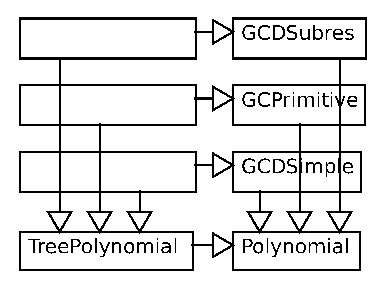
\epsfig{file=Polynomial,clip=,width=0.7\linewidth}
\caption{Polynomial GCD}
\label{fig:poly}
\end{figure}

\subsection{Categories using mixins} % -------------


\begin{verbatim}
class RationalPolynomialCategory(n: Int, vars: Array[String])
  extends PolynomialRing[BigRational](new BigRational(), n, vars)
          with GcdEngineX[BigRational] 
          with SquarefreeEngineZ[BigRational]
          with FactEngineY[BigRational]
\end{verbatim}

\begin{verbatim}
RationalPolynomialCategoryGcdXSqfZFactY
\end{verbatim}

\begin{verbatim}
trait GcdEngineX[C <: RingElem[C]] {
      //??val coFac: RingFactory[C];
      Polynomial[C] gcd(a: Polynomial[C], b: Polynomial[C]) {
                // implementation 
      }
      ...
}
\end{verbatim}

\begin{verbatim}
trait SquarefreeEngineZ[C <: RingElem[C]] {
      //??val coFac: RingFactory[C];
      Polynomial[C] squarefreePart(a: Polynomial[C]) {
                // implementation 
      }
      List[Polynomial[C]] squarefreeFactors(a: Polynomial[C]) {
                // implementation 
      }
      ...
}
\end{verbatim}

\begin{verbatim}
trait FactorEngineY[C <: RingElem[C]] {
      //??val coFac: RingFactory[C];
      List[Polynomial[C]] factorList(a: Polynomial[C]) {
                // implementation 
      }
      SortedMap[Polynomial[C],Long] factors(a: Polynomial[C]) {
                // implementation 
      }
      ...
}
\end{verbatim}

%\begin{verbatim}
%\end{verbatim}

Implementations could be retrieved via factories:
\begin{verbatim}
PolynomialCategoryFactory.<BigRational>getImplementation(coFac)
\end{verbatim}



\section{Conclusions} % --------------------------

To be written


\subsection*{Acknowledgments} %-------------------------

We thank our colleagues Thomas Becker, Wolfgang K. Seiler, Thomas
Sturm, Axel Kramer, Jaime Gutierrez, Sherm Ostrowsky, Ted Kosan and
others for various discussions on the design of and the requirements
for JAS and ScAS. 
%Thanks also to the referees for the insightful suggestions to improve the paper.


\bibliographystyle{splncs}
\bibliography{com-cas}
%\balancecolumns % insert in last page

\end{document}

%%% Local Variables:
%%% mode: latex
%%% TeX-master: t
%%% End:
